\documentclass{report}
\usepackage[utf8]{inputenc}
\usepackage{graphicx}
\usepackage{circuitikz}
\usepackage{pgfplots}
\pgfplotsset{width=10cm,compat=1.9}

\title{Vienkāršu elektrisku
shēmu modelēšana}
\author{Artūrs Pesockis REBC03}
\date{May 2018}

\begin{document}

\maketitle


\chapter{Teorētiska daļa}

Uzdevums: \newline
Apēķiniet spriegumus uz rezistoriem 1. attēlā dotajā shēmā. Sprieguma avota V1 sprieguma
vērtību U (Voltos) izvēlieties daļskaitli, kas būtu Jūsu apliecības pēdējie trīs cipari dalīti ar
10. Piemēram. ‘101REB123’ nozīmē V1 = 12.3 (Volti), R1 ir apliecības pēdējo 3 ciparu otrais
numurs+1, R2 ir apliecības numura pēdējais cipars +1. Piemēram, ja Jūsu apliecības numurs
ir ‘101REB123’ tad ‘R1=3’, ‘R2=4’.\cite{test1} \newline
Variants: \newline
Manas apliecibas numurs ir 171REB104 savukārt V1 pēc formulas būs 10.4 V, R1=0+1 Om, R2=4+1 Om.\cite{test2} \newline


\begin{center}
\begin{circuitikz}[american voltages]
\draw
  (0,0) to [short] (2,0)
  to [R, l_=$R_1$] (4,0)
  to [short] (6,0)
  to [V, l_=$V_1$] (6,4) 
  to [short] (5,4) 
  (0,0) to [short] (0,4) 
  to [short] (1,4) 
  to [R, l_=$R_2$] (3,4)
  to [short] (5,4); 
  \end{circuitikz}
  \end{center}
  \newpage
  
\begin{tikzpicture}
\begin{axis}[
    title={pgfplots grafiks},
    xlabel={R2},
    ylabel={UR2},
    xmin=0, xmax=50,
    ymin=8, ymax=11,
    xtick={0,10,20,30,40,50},
    ytick={9,10},
    legend pos=north west,
    ymajorgrids=true,
    grid style=dashed,
]
\addplot[
    color=blue,
    mark=square,
    ]
    coordinates {
    (0,8.3)(10,9.5)(20,9.8)(30,10.1)(40,10.2)(50,10.25)
    };
\end{axis}
\end{tikzpicture} \newpage

\section{Ķēdes aprēķins}

\begin{tabular}{|c|c|}
\hline     
     R1 & 1 Oms\\
     \hline
     R2 & 5 Oms\\
     \hline
     V1 & 10.4 V \\
     \hline
     U_{R2} & 10.4 V \\
     \hline
     U_{R1} & 8.67 V \\ 
\hline
\end{tabular}

\chapter{Praktiskā daļa}
\section{Darbs ar GEDA programmām}
\subsection{darbs ar gschem}

    \begin{figure}[!htb]
    \centering
        \includegraphics[scale=0.6, angle=180]{1sch}
        \caption{gschem shēma}
        \label{fig:my_label}
    \end{figure} \newpage



\subsection{darbs ar gnetlist}

\begin{verbatim}
* Spice netlister for gnetlist
R2 2 0 5
R1 1 2 1
V1 0 1 10.4
.END

\end{verbatim}

\subsection{darbs ar ngspice}
 \begin{figure}[!htb]
    \centering
        \includegraphics[scale=0.45]{011.ps}
        \caption{R1 grafiks}
        \label{fig:my_label}
    \end{figure} \newpage
    
     \begin{figure}[!htb]
    \centering
        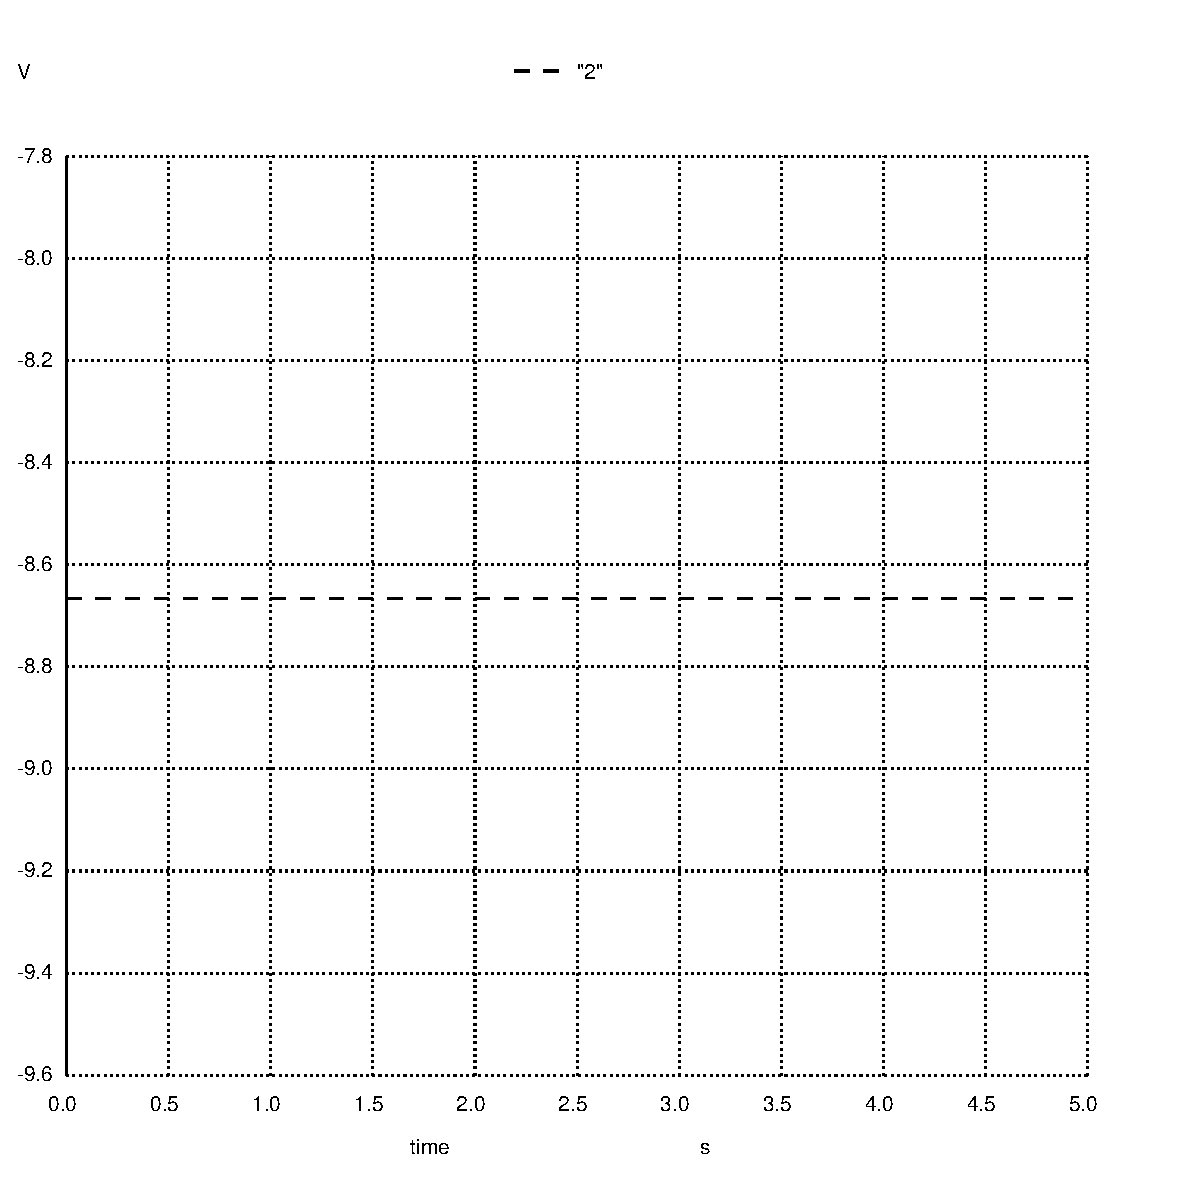
\includegraphics[scale=0.45]{012.ps}
        \caption{R2 grafiks}
        \label{fig:my_label}
    \end{figure} \newpage



\section{Darbs ar QUCS programmām}

    \begin{figure}[!htb]
    \centering
        \includegraphics[scale=0.5]{dc}
        \caption{Shēma QUCS vidē un DC simulacija}
        \label{fig:my_label}
    \end{figure}


    \begin{figure}[!htb]
    \centering
        \includegraphics[scale=0.5, angle=180]{2sch.png}
        \caption{Sweep simulacija}
        \label{fig:my_label}
    \end{figure}
    
    \begin{figure}[!htb]
    \centering
        \includegraphics[scale=0.5, angle=180]{tab.png}
        \caption{Sweep simulacijas grafiks un tabula}
        \label{fig:my_label}
    \end{figure}
\newpage
\renewcommand{\bibname}{Literatūras saraksts}
\begin{thebibliography}{9}
\bibitem{test1} 
Michel Goossens, Frank Mittelbach, and Alexander Samarin. 
\textit{The \LaTeX\ Companion}. 
Addison-Wesley, Reading, Massachusetts, 1993.
 
\bibitem{test2}
Albert Einstein. 
\textit{Zur Elektrodynamik bewegter K{\"o}rper}. (German) 
[\textit{On the electrodynamics of moving bodies}]. 
Annalen der Physik, 322(10):891–921, 1905.
 
\end{thebibliography}

\end{document}
